\documentclass{article}

% if you need to pass options to natbib, use, e.g.:
%     \PassOptionsToPackage{numbers, compress}{natbib}
% before loading neurips_2020

% ready for submission
% \usepackage{neurips_2020}

% to compile a preprint version, e.g., for submission to arXiv, add add the
% [preprint] option:
    \usepackage[preprint]{neurips_2020}

% to compile a camera-ready version, add the [final] option, e.g.:
    % \usepackage[final]{neurips_2020}

% to avoid loading the natbib package, add option nonatbib:
     \usepackage[nonatbib]{neurips_2020}

\usepackage[utf8]{inputenc} % allow utf-8 input
\usepackage[T1]{fontenc}    % use 8-bit T1 fonts
\usepackage{hyperref}       % hyperlinks
\usepackage{url}            % simple URL typesetting
\usepackage{booktabs}       % professional-quality tables
\usepackage{amsfonts}       % blackboard math symbols
\usepackage{nicefrac}       % compact symbols for 1/2, etc.
\usepackage{microtype}      % microtypography
\usepackage{graphicx}

\usepackage{float}

\title{Attention and BERT}

% The \author macro works with any number of authors. There are two commands
% used to separate the names and addresses of multiple authors: \And and \AND.
%
% Using \And between authors leaves it to LaTeX to determine where to break the
% lines. Using \AND forces a line break at that point. So, if LaTeX puts 3 of 4
% authors names on the first line, and the last on the second line, try using
% \AND instead of \And before the third author name.

\author{%
  Eshwar S R \\
  Department of Computer Science and Automation\\
  Indian Institute of Science\\
  \texttt{eshwarsr@iisc.ac.in} \\
  % examples of more authors
  % \And
  % Coauthor \\
  % Affiliation \\
  % Address \\
  % \texttt{email} \\
  % \AND
  % Coauthor \\
  % Affiliation \\
  % Address \\
  % \texttt{email} \\
  % \And
  % Coauthor \\
  % Affiliation \\
  % Address \\
  % \texttt{email} \\
  % \And
  % Coauthor \\
  % Affiliation \\
  % Address \\
  % \texttt{email} \\
}

\begin{document}

\maketitle

\begin{abstract}
  In the recent times, attention based models are out performing LSTM and GRU based networks in a wide range of NLP tasks. Pre-trained models like BERT, RoBERTa etc have achieved state-of-the-art results in many NLP tasks. In this work, I would like to review the basic components of transformers and model architecture of google's BERT model. 
\end{abstract}

\section{Introduction}

Recurrent neural networks, Long short-term memory networks, Gated Recurrent networks were performing very well on sequence based tasks, like language modelling, machine translation, for quite some time and they were the default networks for any sequence based problems. Elmo \cite{peters-etal-2018-deep} was one of the famous model for generating contextual embeddings, which was very popular for quite some time, was based on LSTM networks. The pretrained model was used on many tasks like question answering, textual entailment etc, and it outperformed in many of those tasks. 

Though recurrent networks perform well, they are sequential and take inputs one at a time. This limits us in parallelization during training. However, few factorization tricks \cite{DBLP:journals/corr/KuchaievG17} and conditional computation \cite{NIPS2016_6295} tricks are tried out, the underlying constraint of sequential computation still holds. 

Transformer \cite{vaswani2017attention} model goes away with this sequential computation constraint and uses self attention mechanisms to infer the global dependencies between inputs and the outputs. They are no more sequence based and hence can be parallelized, yielding better results with less training time. Transformer was the first transduction model relying entirely on self-attention to compute representations of its input and output without using sequence aligned RNNs or convolution.

There were some similar attempts made earlier to go away with the sequential dependencies, some of which are Extended Neural GPU \cite{NIPS2016_6295}, ByteNet \cite{DBLP:journals/corr/KalchbrennerESO16} and ConvS2S \cite{DBLP:journals/corr/GehringAGYD17}, all of which use Convolution networks to compute hidden representations for all input and output positions.

BERT \cite{devlin-etal-2019-bert} and other recent models use transformers as basic blocks and are trained on huge corpus. The trained models are shared publicly. These models are then fine tuned as per the task to give state-of-the-art results.

\section{Transformer Model Architecture}
Transformers [\ref{fig:transformer_overview}] follow the basic framework as that of encoder decoder model, where the encoder maps the sequence of symbols into a latent representation of some higher dimensions. Once the representation is found, the decoder uses it to generate a sequence of symbolic outputs in an auto-regressive fashion utilising the previously generated outputs.

\subsection{Encoder and Decoder Stacks}

\textbf{Encoder:} The encoder is typically made up of N=6 blocks stacked one over the other. Each block has two sublayers, first is the multi head self-attention layer followed by a fully connected feed forward network. Both of the sublayers are immediately followed by a layer normalization \cite{ba2016layer} which also take in input from the residual connections \cite{DBLP:journals/corr/HeZRS15}. To facilitate this residual connections all the blocks produce same dimensional output, say $d_{model}$. 

\textbf{Decoder:} The decoder is also typically made up of N=6 blocks stacked one over the other. The sublayers of decoder are similar to that of encoder, but there is an additional layer on top of those two layers to perform multi-head attention over the output from input stack. One more subtle change is the masking of future words to avoid attention towards the unseen words.

\subsection{Attention}
Attention can be well described as a mapping from a query vector to an output vector utilizing a set of key value vectors. A similarity function is used to calculate similarity between the query vector and all the keys, then these similarities are used to calculate the weighted sum of corresponding values to get the final output vector.

\subsubsection{Scaled Dot-Product Attention}
The authors propose an idea called "Scaled Dot-product Attention" [\ref{fig:scaled_dot_product}]. The query and keys are vectors of dimensions $d_k$, and the values are vectors of dimensions $d_v$. The idea is to compute dot products between query and all the keys, divide them by $\sqrt{d_k}$ and then apply softmax to obtain the normalized weights for summing the corresponding values. These computations are parallelized using matrix multiplications. There are two most commonly used attention functions. Additive attention \cite{bahdanau2014neural} which computes the similarity using a feed forward network with single hidden layer. Multiplicative attention is identical to the author's algorithm, except for the scaling factor of $\sqrt{d_k}$.

\subsubsection{Multi-Head Attention}
Instead of performing a single attention, there are multiple heads computing same dimensional output vectors. After which these vectors are concatenated and projected again to get the final output [\ref{fig:multihead_attention}]. Allowing such multiple heads leads the model to attend to different representation subspaces at different positions. There are 3 different places attention is used in transformers. Encoder Decoder Attention allows every position in decoder to attend to every position in encoder sequence. Encoder Attention allows each encoder position to attend to each position of the output from the previous encoder layer. Decoder Attention allows each position in the decoder to attend to all positions in the decoder up to and including that position. Appropriate masking is done to prevent the information leak.

\subsection{Pointwise Feed forward networks}
As illustrated in the figure [\ref{fig:transformer_overview}], every block contains a fully connected feed forward network which is applied to each position separately and identically. This network consists of ReLU activation sandwiched between two linear layers. Each block has its own set of parameters and there is no sharing of parameters as such.

\subsection{Positional Encoding}
As transformer model does not take input in a sequence, the ordering information should be somehow well communicated to the model. There are two ways of doing this positional encoding. These positional encodings are added to the input embeddings at the bottom of encoder and decoder stacks. The positional embeddings can be either learned or fixed \cite{DBLP:journals/corr/GehringAGYD17}. Authors use sine and cosine functions with different frequencies. They also claim that there were no big differences by learning those positional embeddings.

\section{BERT: Bidirectional Encoder Representations from Transformers}

The core idea of BERT is to create a pre-trained language model, which can be fine tuned on tasks to achieve good results even with less data. There are two ways of using pre-trained language models. One such approach is called "feature based", like that of ELMo, which uses task-specific architectures that include the pre-trained representations as additional features. The other way is fine-tuning, like that of BERT, where all or subset of parameters are updated during the training of each task specific model. 

Authors show that the fine-tuned $BERT_{LARGE}$ model produced state-of-the-art results in eleven NLP tasks.

\subsection{Model Architecture}
BERT is completely based on Transformers and its implementation is very much identical to that of the Transformers paper \cite{vaswani2017attention}. 

The authors published two models. Namely, $BERT_{BASE}$ and $BERT_{LARGE}$.
$BERT_{BASE}$ model is similar in size of OpenAI GPT \cite{radford2018improving} another transformer based model, useful for comparison purposes. So, the $BERT_{BASE}$ model consists of 12 layers, each with 12 attention heads and embedding dimension of 768. Where as the $BERT_{LARGE}$ is a very huge model with 24 transformer layers, each with 16 attention heads and embedding dimension of 1024.

\subsection{Input and output representation}
The BERT model is flexible to take single sequence inputs as well as pair of sequences. BERT uses WordPiece \cite{DBLP:journals/corr/WuSCLNMKCGMKSJL16} embedding with a vocabulary size of 30,000 tokens.
There are three important special tokens one should be aware of. [CLS] token which is the first token in any sample fed into the model. The corresponding representation is used for training a classifier on top of BERT during fine tuning. [SEP] token, which is used to differentiate between the pair of sequences in the input. [PAD] token used for padding the sequences to have same length.
Each input representation is sum of its embedding and the positional encoding.

\subsection{Training}
BERT uses bidirectional transformers and is trained on two tasks, namely, masked language modeling(MLM) and next sentence prediction(NSP).

In MLM, the authors mask 15\% of all WordPiece tokens in each sequence at random. If the i-th token is chosen, authors replace the i-th token with (i) the [MASK] token 80\% of the time (ii) a random token 10\% of the time (iii) the unchanged i-th token 10\% of the time. Then, model is trained to predict the original token with cross entropy loss.

In NSP, when choosing the sentences A and B for each pretraining example, 50\% of the time B is the actual next sentence that follows A (labeled as IsNext), and 50\% of the time it is a random sentence from the corpus (labeled as NotNext).

\subsubsection{Dataset}
The pre-training corpus authors used are the BooksCorpus (800M words) \cite{zhu2015aligning} and English Wikipedia (2,500M words).

In Wikipedia data, only text passages were considered leaving out all the other items like headers, lists, tables, html tags etc.

\section{Experiments}
I coded\footnote{Code for all the experiments can be found at: \url{https://github.com/EshwarSR/TransAndBert}} up the transformers using pytorch and ran on IMDB Movie review dataset \cite{maas-EtAl:2011:ACL-HLT2011} which contains 25K train and 25K test samples. Out of the 25K training samples, I used 5K as validation set. 

I tried with a total of 4 transformer architectures. A combination of 8 and 16 heads over 6 and 12 layers trained for 20 epochs.
After that, I also fine-tuned the $BERT_{BASE}$ uncased model over 5 epochs to compare the performances.

\section{Results}

The accuracies are summarized in Table~\ref{accuracies-table}. All the 4 transformer models provide similar results, but the fine tuned $BERT_{BASE}$ model outperforms the other models with a great margin. Please see [\ref{appendix:plots}] for the accuracy plots.

\begin{table}
  \caption{Accuracies on various transformer models. H=heads, L=layers, FT=Fine tuned}
  \label{accuracies-table}
  \centering
  \begin{tabular}{cccccc}
    \toprule
    \cmidrule(r){1-2}
    Model     & 8H 6L    & 8H 12L  & 16H 6L  & 16H 12L  & FT $BERT_{BASE}$  \\
    \midrule
    Train & 0.97 & 0.97 & 0.94 & 0.99 & 0.99  \\
    Valid & 0.77 & 0.77 & 0.77 & 0.78 & 0.94  \\
    Test & 0.76 & 0.76 & 0.76 & 0.76 & 0.93  \\
    \bottomrule
  \end{tabular}
\end{table}



\section{Discussion}

With attention models boosting the performance of many NLP tasks, it has raised a lot of curiosity among researchers related to the interpretability of attention mechanisms. Studies explaining and debugging the current system's decision \cite{lee-etal-2017-interactive} and  distilling important traits of a dataset \cite{yang-etal-2017-satirical} are also carried out. Authors of "Is Attention Interpretable?" \cite{serrano2019attention} feel attention weights are only noisy predictors of even intermediate components' importance, and should not be treated as justification for a decision. They claim that in order for a model to be interpretable, it must not only suggest explanations that make sense to people, but also ensure that those explanations accurately represent the true reasons for the model's decision. They conclude that while attention noisily predicts input components' overall importance to a model, it is by no means a fail-safe indicator. 

The work "Attention is not explanation" \cite{jain2019attention} performs extensive experiments across a variety of NLP tasks (like text classification, natural language inference (NLI), and question answering) that aim to assess the degree to which attention weights provide meaningful "explanations" for predictions. That authors find that they largely do not. The authors also propose an approach to counterfactual attention weights called "adversarial attention".

The work "Attention is not not explanation" \cite{wiegreffe2019attention} is another work challenging the claims of the previously mentioned work \cite{jain2019attention}. The authors propose four alternative tests to determine when/whether attention can be used as explanation: a simple uniform-weights baseline; a variance calibration based on multiple random seed runs; a diagnostic framework using frozen weights from pretrained models; and an end-to-end adversarial attention training protocol. Each of which allows for meaningful interpretation of attention mechanisms in RNN models.

Similar works are done in trying to understand the Geometry of BERT \cite{DBLP:journals/corr/abs-1906-02715} too. The authors show that the BERT model does good job with respect to word senses. They shown how mistakes in word sense disambiguation may correspond to changes in internal geometric representation of word meaning. They run experiments to show that BERT has both syntactic (particularly, dependency relations) and semantic subspaces. They claim that the internal geometry of BERT may be broken down into multiple linear
subspaces, with separate spaces for different syntactic and semantic information.

Irrespective of the interpretability of attention, the truth is that these transformer based models have created a new benchmark in the domain of NLP. In the present crisis of the Covid-19 pandemic, these models are helping fight spread of misinformation and in retrieval of right information too.
Some of the related work are, "An Analysis of BERT FAQ Retrieval Models for COVID-19 Infobot"\footnote{\url{https://openreview.net/forum?id=dGOeF3y_Weh}}, model to analyse COVID-19 Content on Twitter using BERT \cite{mller2020covidtwitterbert} and CrisisBERT \cite{liu2020crisisbert}, a classifier of crisis events, such as natural disasters, terrorist attacks and pandemics.

\bibliography{neurips_2020.bib}
\bibliographystyle{nips}
\appendix
\section*{Appendix}
\section{Figures}
The following images are taken from the original transformer paper \cite{vaswani2017attention}.

% \begin{minipage}{0.4\textwidth}
%  \centering
%  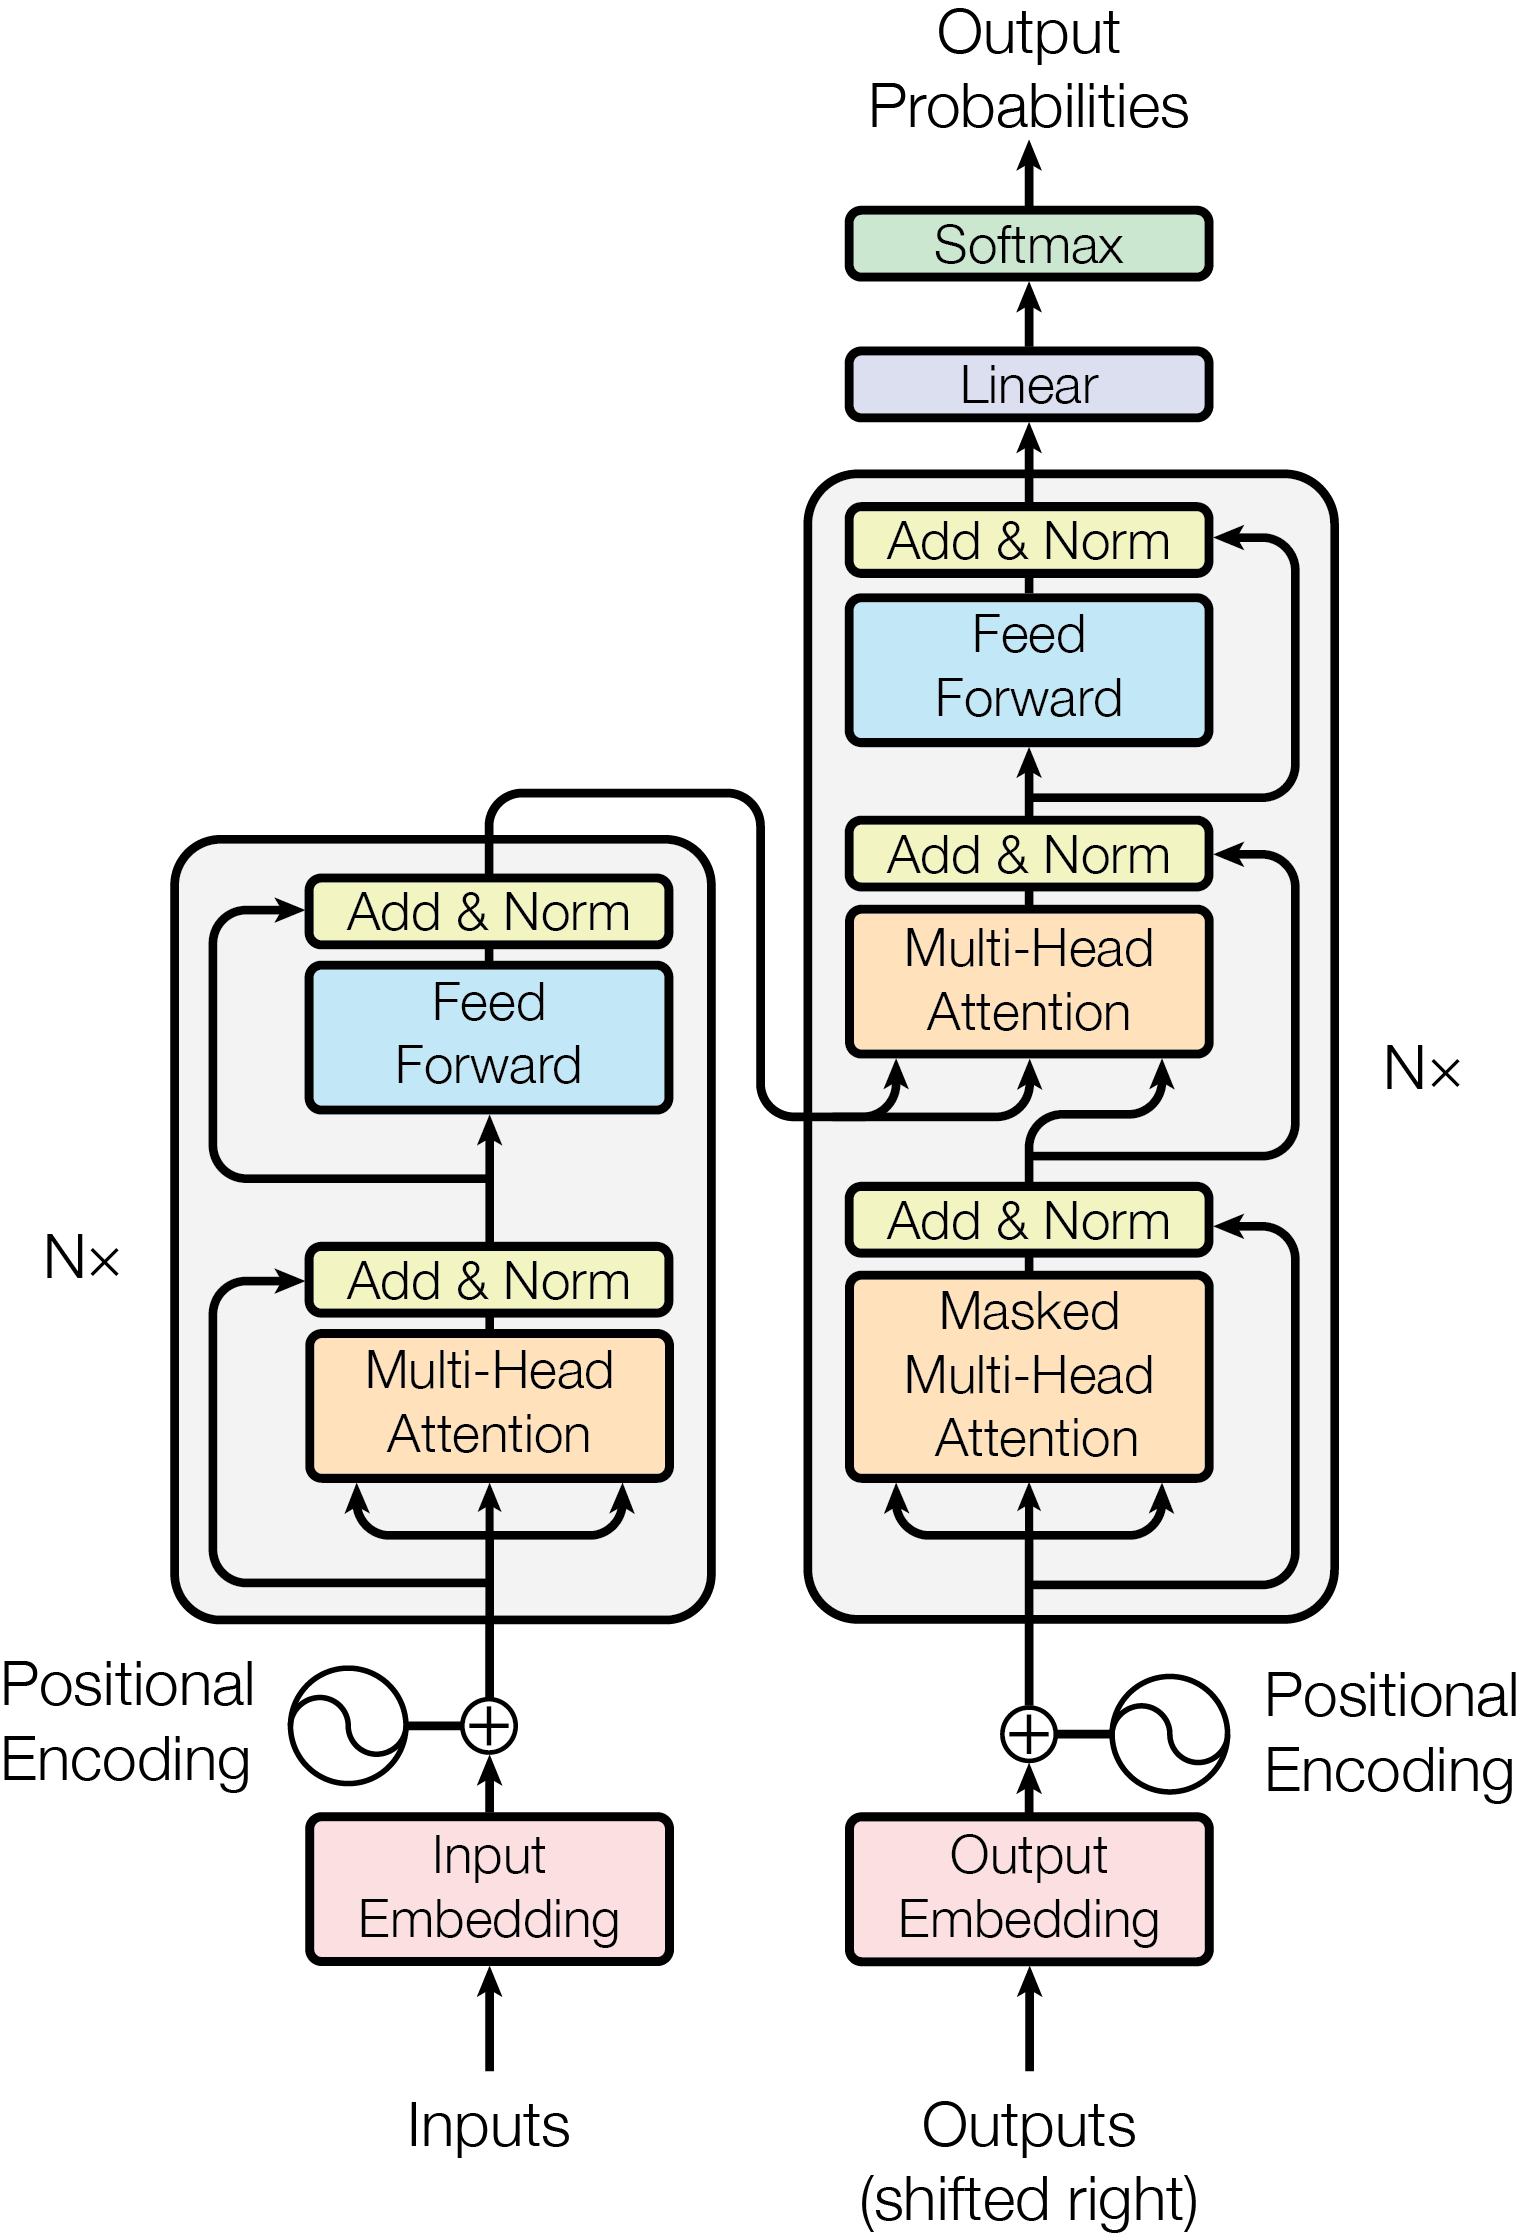
\includegraphics[width=1\linewidth]{Transformer.png}
%  \caption{Overview of Transformer Architecture}
%  \label{fig:transformer_overview}
% \end{minipage}\hfill

\begin{figure}[H]
    \centering
    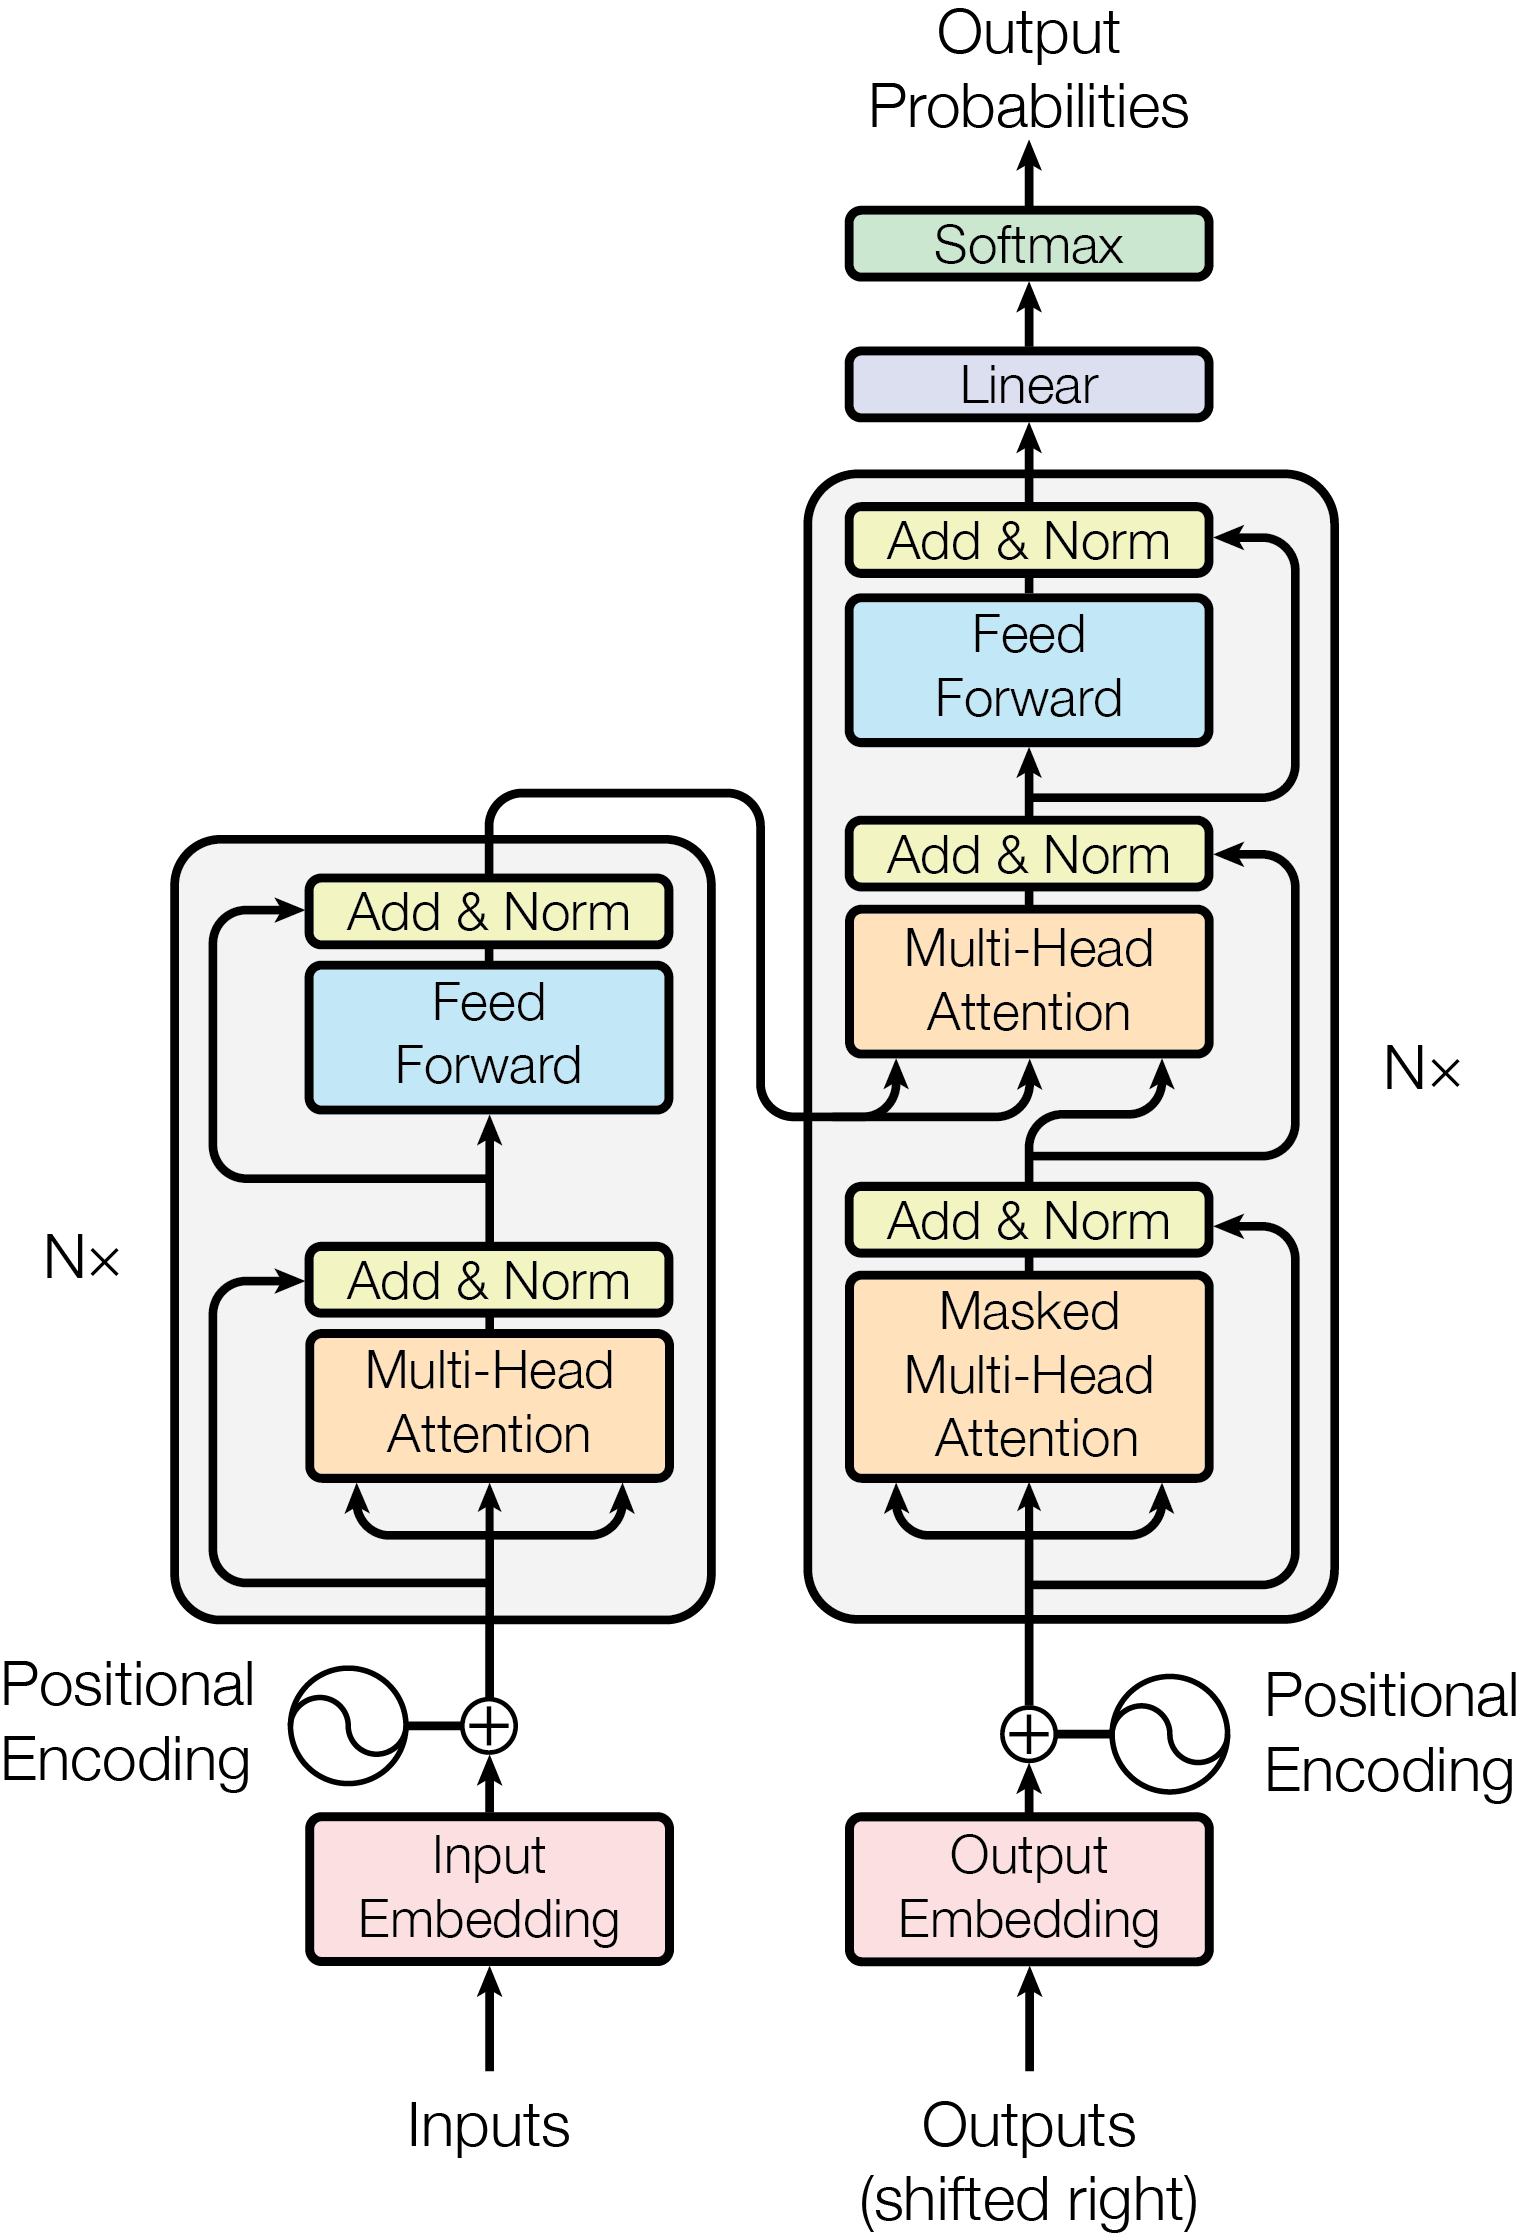
\includegraphics[scale=0.27]{Transformer.png}
    \caption{Overview of Transformer Architecture}
    \label{fig:transformer_overview}
\end{figure}

% \begin{figure}[H]
%     \centering
%     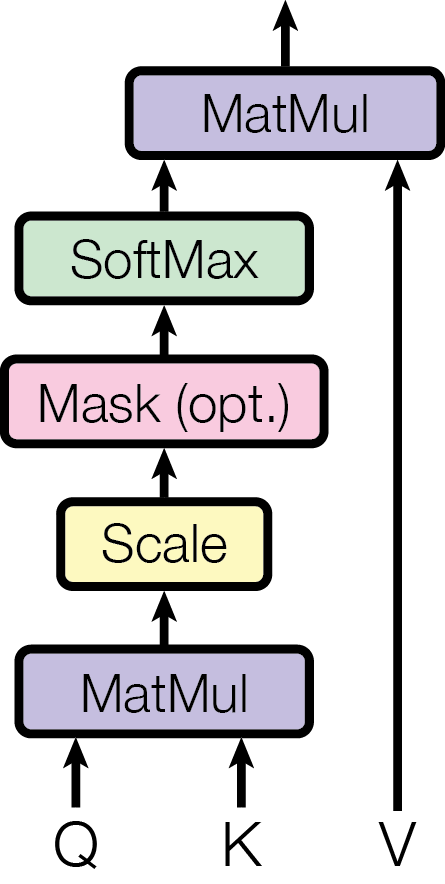
\includegraphics[scale=0.27]{dot_product.png}
%     \caption{Scaled Dot Product}
%     \label{fig:scaled_dot_product}
% \end{figure}

% \begin{figure}[H]
%     \centering
%     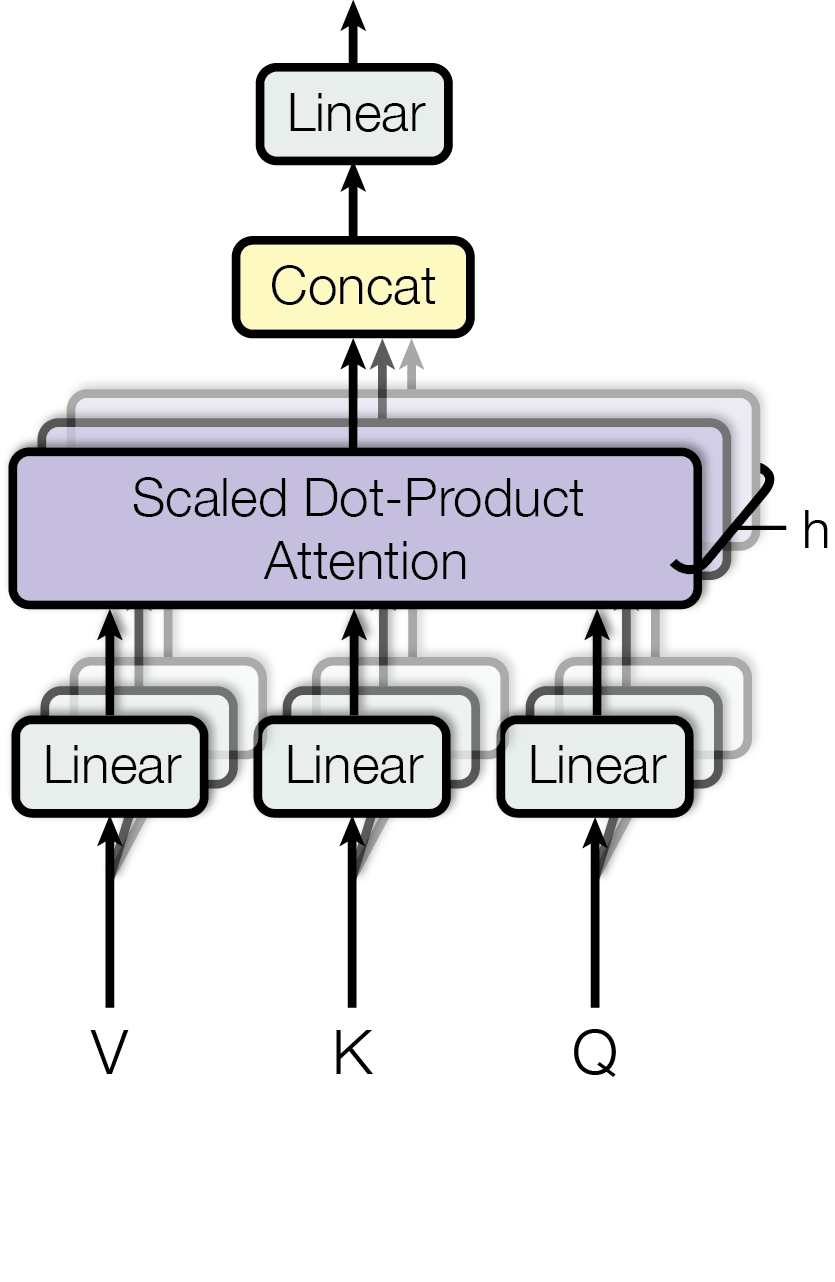
\includegraphics[scale=0.27]{Multihead attention.png}
%     \caption{Multihead attention}
%     \label{fig:multihead_attention}
% \end{figure}

\begin{minipage}{0.35\textwidth}
 \centering
 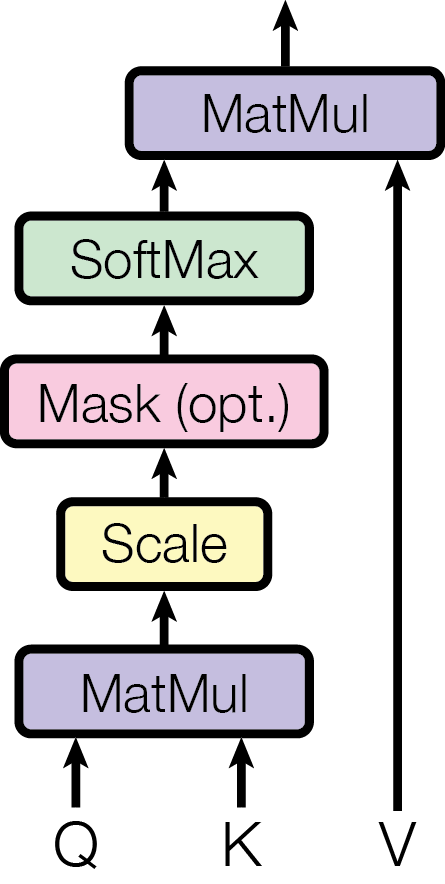
\includegraphics[width=1\linewidth]{dot_product.png}
 \caption{Figure 2: Scaled dot product}
 \label{fig:scaled_dot_product}
\end{minipage}\hfill
\begin{minipage}{0.49\textwidth}
 \centering
 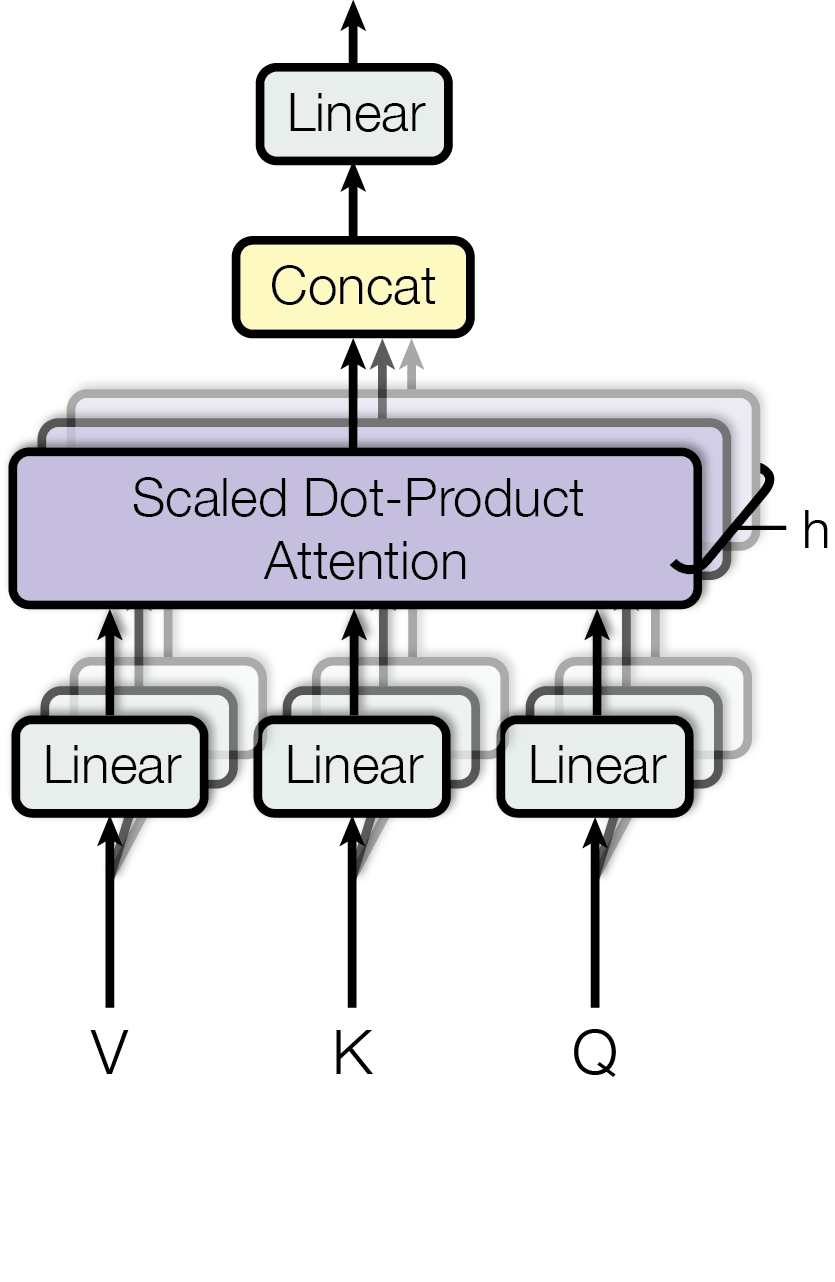
\includegraphics[width=1\linewidth]{Multihead attention.png}
 \caption{Figure 3: Multihead attention}
 \label{fig:multihead_attention}
\end{minipage}\hfill

\section{Plots}
\label{appendix:plots}
Below are the training and validation accuracy plots against each epoch for the models of Table \ref{accuracies-table}. \\
\begin{minipage}{0.49\textwidth}
 \centering
 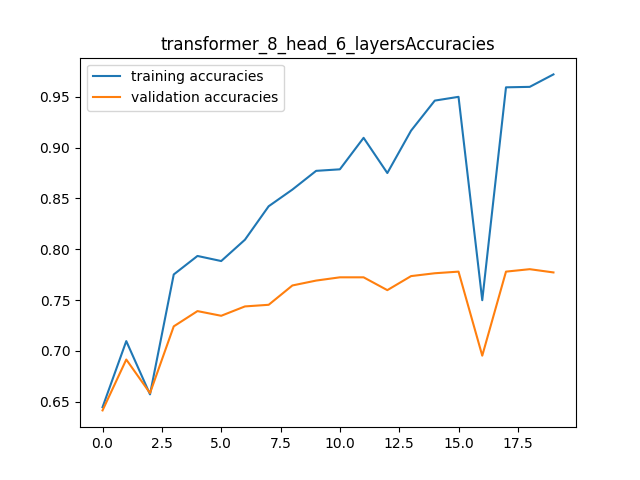
\includegraphics[width=1\linewidth]{transformer_8_head_6_layers_Accuracies.png}
 \caption{Accuracies of 8 heads 6 layered model}
\end{minipage}\hfill
\begin{minipage}{0.49\textwidth}
 \centering
 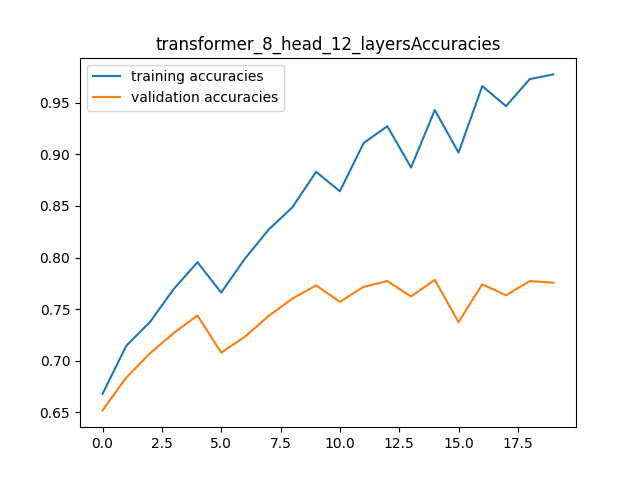
\includegraphics[width=1\linewidth]{transformer_8_head_12_layers_Accuracies.png}
 \caption{Accuracies of 8 heads 12 layered model}
\end{minipage}\hfill
\begin{minipage}{0.49\textwidth}
 \centering
 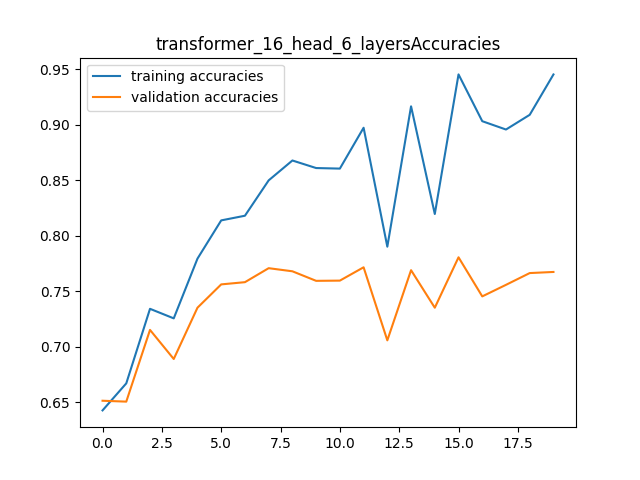
\includegraphics[width=1\linewidth]{transformer_16_head_6_layers_Accuracies.png}
 \caption{Accuracies of 16 heads 6 layered model}
\end{minipage}\hfill
\begin{minipage}{0.49\textwidth}
 \centering
 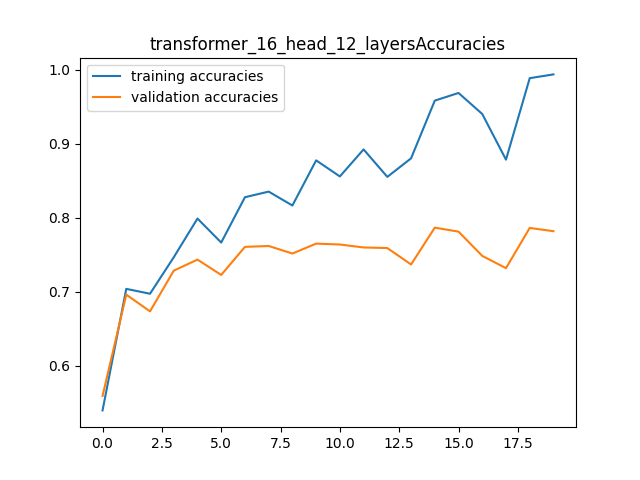
\includegraphics[width=1\linewidth]{transformer_16_head_12_layers_Accuracies.png}
 \caption{Accuracies of 16 heads 12 layered model}
\end{minipage}\hfill
\begin{minipage}{0.49\textwidth}
 \centering
 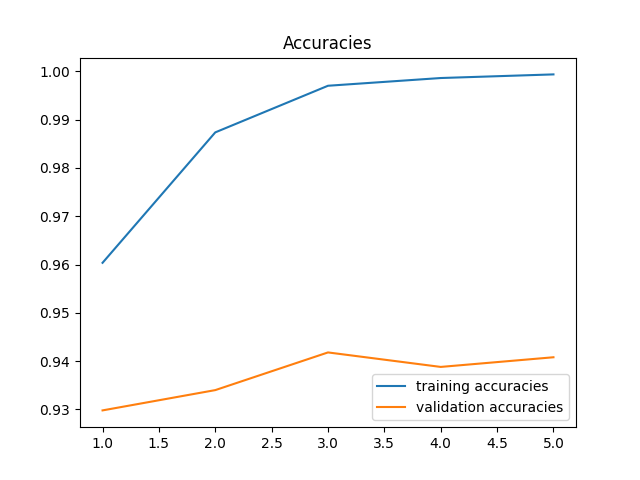
\includegraphics[width=1\linewidth]{BERT_Accuracies.png}
 \caption{Accuracies of fine-tuned BERT}
\end{minipage}\hfill

\end{document}